\noindent
\textbf{Proposed Tasks.}
We propose the following Tasks to realize a multiscale simulation
capability within Nek5000/RS/ROM for reactor analysis.
%% , following the schedule laid out in Fig.~\ref{fig:gantt}. 
\\[-2ex]

\noindent
\textbf{Task 1: Data Generation.} We will perform high fidelity simulations of 
the flow in SFR fuel assemblies (e.g., Fig. \ref{fig:sum}, left), including 
a range of steady-state conditions and a loss-of-flow transient scenario.
\\[-4ex]
\begin{description}
\item{$\; i.$}
Define benchmarks for SFR fuel assemblies. These will be used for validation.
\\[-4ex]
\item{$\, ii.$}
Develop data to construct ROMs for SFR fuel assemblies. This
task will support Task 2.  
\\[-4ex]
\item{\em iii.} Develop data to validate ROMs for both
transient and parameter sweeps to support Task 3.
\\[-3ex]
\end{description}
In Task 1, we will leverage several cases developed as benchmarks for mixed
convection and thermal striping as part of a recent IRP. The cases are
summarized in Table~\ref{tab:cases}. For this project, we will augment these
cases by performing simulations for a broader range of parameters and
collecting additional snapshots as needed. We remark that using well-defined
past benchmarks also allows us to evaluate the performance advantage of
ROM-based approaches. \\[-2ex]

\begin{table}
\centering
\begin{tabular}{|l|c|c|c|}
\hline
\textbf{Case} & \textbf{Size} (grid points) & \textbf{Run time} (CU) & \textbf{Snapshots} \\\hline
Mixed convection (19 pins) \cite{kraus22}& $1\cdot 10^{9}$ & 20,000 & 5000 \\
\hline
Mixed convection (61 pins) \cite{kraus22}& $3\cdot 10^{9}$ & 2000 &  5000 \\
\hline
Parallel Jets \cite{acierno22}& $1\cdot 10^{9}$ & 200,000 & 10,000 \\
\hline
Thermal stratification \cite{krohn2018} & $5\cdot 10^{8}$ & 500,000 & 10,000 \\
\hline
\end{tabular}
\caption{\label{tab:cases} List of existing cases.}
\end{table}

% \begin{figure}[b!] \centering
%    {\setlength{\unitlength}{1.0in} \begin{picture}(6.5,2.500)(0.0,0)
%      \put(0.9,-.00){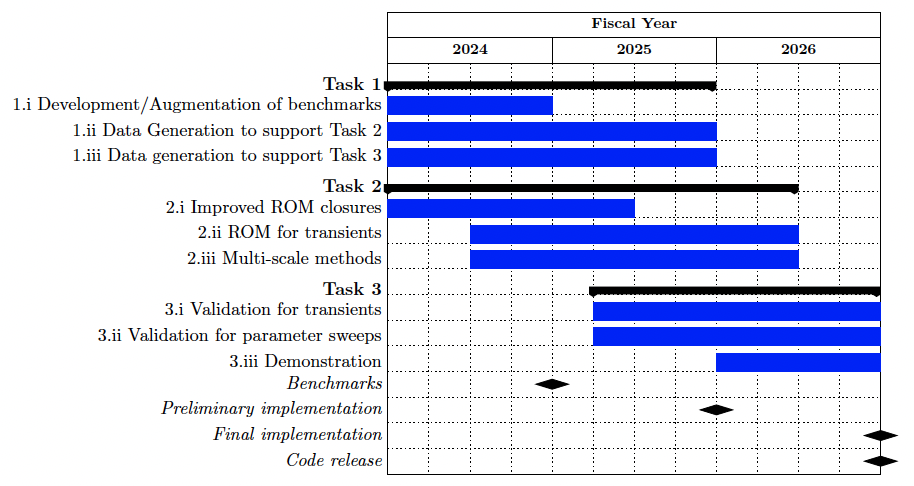
\includegraphics[height=2.7in]{figs/neup_gantt_v1.png}}
%    \end{picture}} 
%    \caption{Timeline of proposal by fiscal year.  \label{fig:gantt}
% \\[-2ex]
% }
% \end{figure}


\noindent
\textbf{Task 2: Algorithmic Development.} This is the core of the project.
We seek to develop advanced ROM methods that are seemlessly
extended to a multi-scale framework in Nek5000/RS/ROM.
\\[-4ex]
\begin{description}
\item{$\; i. \; \; \;$}
Continued development of ROM closure models to increase robustness 
for high Rayleigh/Reynolds flows.  This effort will build on earlier and 
ongoing work
\cite{kaneko22a,kaneko22,tsai22a,kaneko20a,mou2021}.
\\[-3ex]
\item{$\, ii. \;\;$}
Identify strategies to equip the ROM for long-time transients.  
Proposed extensions to \cite{kaneko20a} include employing error indicators
developed in \cite{fick18,tsai22a} for transients and development of 
LES-based filter-based stabilization methods in the context of ROMs.
\\[-3ex]
\item{\em iii. \;}Develop multi-scale methods that couple ROMs with LES on a 
subset of the domain, as illustrated in Fig. \ref{fig:cha1}(right).
A principal challenge is to quantify the relaxation distances over which small
scale structures will evolve near the ROM-LES interface. The goal will be to
combine reactor-scale ROM simulations with localized detailed simulations in
regions of interest. This task leverages past work on rod bundles and sub-channels,
whose geometric properties have been exploited to maximize the use of 
small-domain high-fidelity simulation to improve RANS results in a multi-scale
fashion \cite{martinez2019a}.  
\\[-3ex]
\end{description}%

\noindent
\textbf{Task 3: Validation and Demonstration.} 
Here we validate and demonstrate the proposed methods.
\\[-4ex]
\begin{description}
\item{$\; i.\; \;$}
Validate ROM transient calculations with high-fidelity counterparts
in an SFR rod-bundle under \textit{low-flow} conditions.
\\[-4ex]
\item{$\, ii. \,\;$}
Perform ROM-based parameter sweeps and compare with corresponding
FOM data for validation.
\\[-4ex]
\item{\em iii.}
Demonstrate accelerated transient capability for cases that are currently not
feasible. We will implement the proposed ROM-based and multiscale models within
Cardinal \cite{cardinal}. This will enable their usage within the systems
analysis code SAM \cite{hu2021}. The co-PI at Penn State has been working
extensively on the integration of SAM and NekRS within Cardinal.
\\[-3ex]
\end{description}
Below, we describe subtasks to be addressed in support of the main Tasks
outlined above.
\newpage
